% vim: set tw=78 sts=2 sw=2 ts=8 aw et ai:
\documentclass{workshop}

% Comentează liniile de mai jos în cazul în care nu există cod de inclus.
\usepackage{code/highlight}
\usepackage{color}        % dacă e folosit highlight
\usepackage{alltt}        % dacă e folosit highlight

\title[Sesssion 10]{Session 10}
\subtitle{Contributing to Upstream: GIT Versioning, Patching, Linux Community}
\author{Daniel Băluță, Irina Preșa}
\date{13 July 2012}

\begin{document}

% Arătăm numărul frame-ului
\setbeamertemplate{footline}[frame number]

\frame{\titlepage}

% NB: Secțiunile nu sunt marcate vizual, ci doar apar în cuprins
\section{GIT Versioning Control}

\begin{frame}{GIT Versioning Control}
\begin{itemize}
\item version control software started by Linus Torvalds.
\item high performance for maintaining large projects.
\item<2> "git" $=$ English slang for a stupid or unpleasant person.
\item<2> Torvalds quipped about the name: \emph{"I'm an egotistical bastard, and I
name all my projects after myself. First 'Linux', now 'git'"}.
\end{itemize}
\end{frame}

\begin{frame}{Why Version Control}
\begin{itemize}
\item restore a previous version.
\item collaborative work.
\item history (comments, changes).
\item branching.
\end{itemize}
\end{frame}

\begin{frame}{Why GIT}
\begin{itemize}
\item increased performance for large projects.
\item distributed (local vs remote repo).
\item third-party tools/applications integration.
\item track/follow remote repos/branches.
\end{itemize}
\end{frame}

\begin{frame}{Repository Architecture}
\begin{figure}
  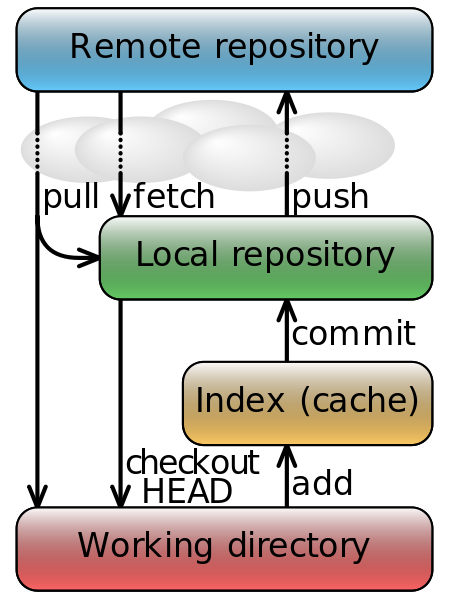
\includegraphics[scale=0.3]{img/flow.png}
\end{figure}
\end{frame}

\begin{frame}{Initial Configurations}
\end{frame}

\begin{frame}{General Operations}
\end{frame}

\begin{frame}{General Flow}
\end{frame}

\begin{frame}{Repo Visualization}
\end{frame}

\begin{frame}{Solving Conflicts}
\end{frame}

\begin{frame}{Patching Solutions}
\end{frame}

\begin{frame}{Extra: Post-Receive Hooks}
\end{frame}

\section{Keywords}

\begin{frame}{Keywords}
     \begin{itemize}
	\item git
      \end{itemize}
\end{frame}

\section{Resources}
\begin{frame}{Resources}
  \begin{itemize}
  \item \href{http://cscope.sourceforge.net/cscope_vim_tutorial.html}{Using Cscope with vim}
  \end{itemize}
\end{frame}

\section{Questions}

\end{document}
